\documentclass[master=elt,masteroption=eg,english]{kulemt}
\setup{% Verwijder de "%" op de volgende lijn bij UTF-8 karakterencodering
  %inputenc=utf8,
  title={The best master's thesis ever},
  author={Een Auteur\and Tweede Auteur},
  promotor={Prof.\,dr.\,ir.\ Weet Beter},
  assessor={Ir.\,W. Eetveel\and W. Eetrest},
  assistant={Ir.\ A.~Assistent \and D.~Vriend}}
% Verwijder de "%" op de volgende lijn als je de kaft wil afdrukken
%\setup{coverpageonly}
% Verwijder de "%" op de volgende lijn als je enkel de eerste pagina's wil
% afdrukken en de rest bv. via Word aanmaken.
%\setup{frontpagesonly}

% Kies de fonts voor de gewone tekst, bv. Latin Modern
\setup{font=lm}

% Hier kun je dan nog andere pakketten laden of eigen definities voorzien

% Tenslotte wordt hyperref gebruikt voor pdf bestanden.
% Dit mag verwijderd worden voor de af te drukken versie.
\usepackage[pdfusetitle,colorlinks,plainpages=false]{hyperref}

%%%%%%%
% Om wat tekst te genereren wordt hier het lipsum pakket gebruikt.
% Bij een echte masterproef heb je dit natuurlijk nooit nodig!
\IfFileExists{lipsum.sty}%
 {\usepackage{lipsum}\setlipsumdefault{11-13}}%
 {\newcommand{\lipsum}[1][11-13]{\par Hier komt wat tekst: lipsum ##1.\par}}
%%%%%%%

%\includeonly{chap-n}
\begin{document}

\begin{preface}
  I would like to thank everybody who kept me busy the last year,
  especially my promoter and my assistants. I would also like to thank the
  jury for reading the text. My sincere gratitude also goes to my wive and
  the rest of my family.
\end{preface}

\tableofcontents*

\begin{abstract}
  The \texttt{abstract} environment contains a more extensive overview of
  the work. But it should be limited to one page.

  \lipsum[1]
\end{abstract}

\begin{abstract*}
  In dit \texttt{abstract} environment wordt een al dan niet uitgebreide
  Nederlandse samenvatting van het werk gegeven.
  Wanneer de tekst voor een Nederlandstalige master in het Engels wordt
  geschreven, wordt hier normaal een uitgebreide samenvatting verwacht,
  bijvoorbeeld een tiental bladzijden. 

  \lipsum[1]
\end{abstract*}

% Een lijst van figuren en tabellen is optioneel
%\listoffigures
%\listoftables
% Bij een beperkt aantal figuren en tabellen gebruik je liever het volgende:
\listoffiguresandtables
% De lijst van symbolen is eveneens optioneel.
% Deze lijst moet wel manueel aangemaakt worden, bv. als volgt:
\chapter{List of Abbreviations and Symbols}
\section*{Abbreviations}
\begin{flushleft}
  \renewcommand{\arraystretch}{1.1}
  \begin{tabularx}{\textwidth}{@{}p{12mm}X@{}}
    LoG   & Laplacian-of-Gaussian \\
    MSE   & Mean Square error \\
    PSNR  & Peak Signal-to-Noise ratio \\
  \end{tabularx}
\end{flushleft}
\section*{Symbols}
\begin{flushleft}
  \renewcommand{\arraystretch}{1.1}
  \begin{tabularx}{\textwidth}{@{}p{12mm}X@{}}
    42    & ``The Answer to the Ultimate Question of Life, the Universe,
            and Everything'' according to \cite{h2g2} \\
    $c$   & Speed of light \\
    $E$   & Energy \\
    $m$   & Mass \\
    $\pi$ & The number pi \\
  \end{tabularx}
\end{flushleft}

% Nu begint de eigenlijke tekst
\mainmatter

\chapter{Introduction}
\label{cha:intro}
The first contains a general introduction to the work. The goals are
defined and the modus operandi is explained.

\section{Lorem Ipsum 4--5}
\lipsum[4-5]

\section{Lorem Ipsum 6--7}
\lipsum[6-7]

%%% Local Variables: 
%%% mode: latex
%%% TeX-master: "thesis"
%%% End: 


\chapter{Initial exploration}
\label{cha:1}
In this chapter an initial exploration of the problem is done. This was done in MATLAB with the neural network toolbox for the backpropagation algorithm, and YALMIP with fmincon for the simultaneous approach.

TODO version numbers, hardware

\section{First experiment}
The first experiment conducted was to apply both algorithms to a test problem. A small neural network is constructed with 2 hidden layers with each layer containing 3 nodes with tansig activation function. The activation function was chosen because it works well for a small network. This network is then trained to approximate a piece of a sine function. Both algorithms are trained for 100 epochs. Figure \ref{} shows the training performance for a training run of each algorithm. Both perform well, but the simultaneous approach is much slower. This can be due to the fact that the new algorithm is not well optimized.

\begin{figure}
     \centering
     \begin{subfigure}[b]{0.8\textwidth}
         \centering
         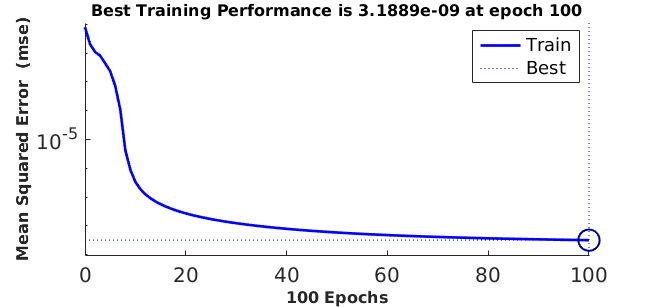
\includegraphics[width=\textwidth]{back_test_1}
         \caption{Training performance of backpropagation}
         \label{fig:y equals x}
     \end{subfigure}
     \begin{subfigure}[b]{0.8\textwidth}
         \centering
         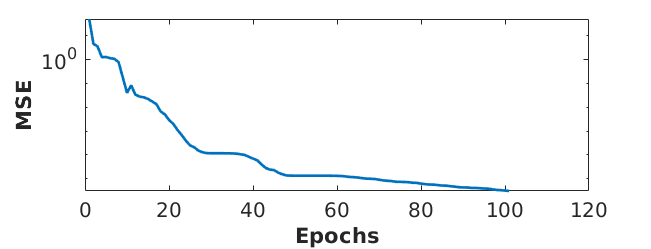
\includegraphics[width=\textwidth]{back_test_12}
         \caption{Training performance of simultaneous approach}
         \label{}
     \end{subfigure}
     \begin{subfigure}[b]{0.8\textwidth}
         \centering
         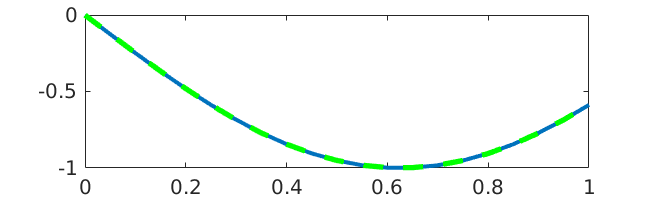
\includegraphics[width=\textwidth]{sine}
         \caption{Sine function}
         \label{}
     \end{subfigure}
        \caption{Performance of algorithms for simple regression problem}
        \label{fig:three graphs}
\end{figure}




The backpropagation algorithm converges every time for this problem, taking anywhere between 10 and 1000 iterations. The stopping criteria is that the validation error increases for 6 consecutive iterations.

The simultaneous approach also converges if the intial conditions are set correctly. The weight variables are randomly initialized and the state variables are initialized by simulating the network once using the input vector, so the initial point is feasible. Letting fmincon run for 200 iterations gives a good solution every time, but the algorithm runs much slower. Its not known if this is due to the difference in optimization of the algorithms and the fact that the backpropagation algorithm is running on my GPU instead of the CPU.

\section{Second experiment}
TODO make it more scientific.

For this experiment the same test problem is considered but with a different network. Here a shallow network 1 layer deep and 10 neurons wide is considered, with the ReLU activation function.

The backpropagation function will sometimes get stuck in a bad solution while training this network, but usually finds a good approximation.

For the simultaneous approach the RELU constraints will have to be reformulated. The ReLU function can be transformed into smooth constraints as follows:

   \begin{gather*}
   x_{k+1}^j = \max(W_kx_k^j,0) \\
   \Updownarrow \\
   x_{k+1}^j = -\min(-W_kx_k^j,0) \\
   \Updownarrow \\
   \min(x_{k+1}^j-W_kx_k^j) = 0 \\
   \Updownarrow \\
   (x_{k+1}^j-W_kx_k^j)^\top x_{k+1}^j = 0,\\
   x_{k+1}^j\geq 0,x_{k+1}^j-W_kx_k^j\geq 0
   \end{gather*}
   
Even using these smooth constraints, the algorithm very often gets stuck in a bad local minimum.
\section{Further exploration}
There are many options that can be explored to further compare these algorithms.

\begin{itemize}
\item Activation function: ReLU is the most popular activation function in the field. Others are tansig, sigmoid, SoftPlus, leaky ReLU, etc.
\item Network size: Networks can be up to thousands of neurons wide and hundreds of layers deep. 
\item Network architecture: There is a huge variety of possible network architectures. Convolutional neural networks for example are very popular for image recognition.
\item Test problems: Neural networks have many applications. Some applications could benefit more from this training method than others.
\item Optimization algorithm: fmincon is quite a general method, a more specific method might perform better
\item Stopping criteria and initial conditions

These will be explored in the next chapters

\end{itemize}




%%% Local Variables: 
%%% mode: latex
%%% TeX-master: "thesis"
%%% End: 

\chapter{Augmented Lagrangian Method}
\label{cha:2}
In this chapter the direct multiple shooting approach is examined more closely and a more specific algorithm is designed to replace \texttt{fmincon}, which is a very general method. For this problem the Augmented Lagrangian Method has been chosen. This is a common method for solving constrained Non Linear Programs (NLPs). Instead of using the classical method, an Augmented Lagrangian framework is adapted from a recent paper\cite{sahin2019}.It will be implemented in python using \texttt{numpy},\texttt{scipy}, and \texttt{keras}.

\section{Classical Augmented Lagrangian Method}
The Augmented Lagrangian Method (ALM) is a classical algorithmic framework for solving constrained NLPs. It was first discovered in 1969 \cite{Hestenes1969},\cite{Powell1969} and was known as the method of multipliers. The textbook examples of this method can be found in \cite{Birgin2009} and \cite{bertsekas2014constrained}.

It is designed to minimize equality constrained optimization problems defined in the following way:

\begin{equation}
	\begin{aligned}
	& \underset{u}{\text{min}} & f(u) & \\
	& \text{s.t.} & h(u) &= 0 \\
	\end{aligned}
\end{equation}

ALM solves this by minimizing a series of unconstrained problems in a similar manner as the penalty method. In each iteration a $\beta$-augmented Lagrangian $\mathcal{L}_\beta(x,\lambda)$ is minimized for x:

\begin{equation}
	\underset{u}{\text{min}} \hspace{.5em} \underset{\lambda}{\text{max}} \hspace{.5em}  \mathcal{L}_\beta(u,\lambda) = f(u) + \langle\lambda,h(u)\rangle + \frac{\beta}{2} || h(u) ||^2_2
\end{equation}

where $\beta>0$ is the penalty weight. This can be viewed as a penalty method which has been shifted using the term in $\lambda$\cite{Birgin2009}. When $\beta$ or $\lambda$ tend to infinity, $h(u)$ will be forced to zero, leading the Lagrangian to converge to the same solution as the original problem.

The algorithm proceeds as follows:
\begin{gather*}
	u_{k+1} = \underset{u}{\text{argmin}} \hspace{.5em} \mathcal{L}_\beta(u,\lambda_k) \\
	\lambda_{k+1} = \lambda_k + \sigma_k h(u_{k+1})
\end{gather*}

where $\sigma_k$ is the step size at iteration $k$. Then in each step the penalty parameter $\beta_k$ is increased or kept the same, depending on the size of the constraint violation. This continues until an acceptable solution has been found:

\begin{equation}
	||h(u_k)|| \leq \tau_1 \hspace{.5em}\text{and}\hspace{.5em} ||\nabla_u\mathcal{L}_{\beta_k}(u_k,\lambda_k)|| \leq \tau_2
\end{equation}

with $\tau_1,\tau_2$ the chosen tolerances.

\section{Applied Augmented Lagrangian Method}

The OCP equation \ref{ocp-eq} of training a neural net with MSE loss function is a constrained nonlinear least squares(LS) problem:
\begin{equation*}
	\begin{aligned}
	& \underset{W}{\text{minimize}}
	& & \sum\limits_{j=0}^{n}||\sigma_L(W_Lz_L) - y_j||^2_2 \\
	& \text{subject to}
	& & z_{1,j} = \sigma_0(W_0,x_j), &j = 1,\ldots,n \\
	& & & z_{k+1,j} = \sigma_k(W_kz_{k,j}), &k = 1,\ldots,L-1,j = 1,\ldots,n \\
    & & \Updownarrow \\
	& \text{min}
	&  & \frac{1}{2} ||F(u)||^2_2 \\
	& \text{s. t.}
	& &  h(u) = 0
	\end{aligned}
\end{equation*}
Where $u = \{W,z\}$ is the collection of both the weight and state variables into a single vector.

The subproblem that will be solved in each iteration is then:
\begin{equation}
	\begin{aligned}
	 & \underset{u}{\text{argmin}} & \mathcal{L}_{\beta}(u,\lambda) 
	     &= \frac{1}{2} ||F(u)||^2_2 + \langle\lambda,h(u)\rangle + \frac{\beta}{2} || h(u) ||^2_2 \\
	 & & &= \frac{1}{2} ||F(u)||^2_2 + \frac{\beta}{2} ||h(u) + \lambda/\beta ||^2_2 - \frac{1}{2\beta} ||\lambda||^2_2 \\
	 & & &= \frac{\beta}{2} \Big|\Big|
		\begin{bmatrix}
			F(u)/\sqrt{\beta} \\
			h(u) + \lambda/\beta
		\end{bmatrix} \Big|\Big|^2_2 \\
	\end{aligned}
	\label{loss}
\end{equation}

Instead of using the textbook algorithm, an algorithmic framework from a more recent paper\cite{sahin2019} is adapted to the problem, shown in Algorithm \ref{algo}.

\begin{algorithm}[H]
\SetAlgoLined
\SetKw{Kw}{Initialization}
\SetKwComment{Comment}{}{}
\SetCommentSty{emph}
\KwIn{Initial weights vector $W$, penalty parameter $\beta$, stopping tolerance $\tau$, input-target pairs $(x_i,y_i), i = 1,\ldots,n$}
\Kw{$u_0 = \{W,f_{W}(x)\}, \lambda_0 \in \mathcal{N}(0,1)$}
\Comment*[r]{Initialize state variables by simulating network, initialize dual variables randomly}
\For{k = 0,1,...}{
 	$\eta_k = 1/\beta^k$
 	\Comment*[r]{Update tolerance}
 	find $u_{k+1}$ such that \\
 	\Indp$||\nabla_{u_k}\mathcal{L}_{\beta^k}(u_k,\lambda_k)|| \leq \eta_k$ \label{ls-prob}
 	\Comment*[r]{Approx. primal solution}
 	\Indm$\sigma_{k+1} = \text{min}\big(\frac{||h(u_0)||\log^22}{||h(u_{k+1})||k \log^2(k+1)},1\big)$
 	\Comment*[r]{Update dual step size}
 	$\lambda_{k+1} = \lambda_k + \sigma_{k+1}h(u_{k+1})$
 	\Comment*[r]{Update dual variables}
 	$||\nabla_{u_{k+1}}\mathcal{L}_{\beta^k}(u_{k+1},\lambda_k)|| + ||h(u_{k+1})||<\tau$
 	\Comment*[r]{Stopping Criterion}
 	
 }
 \caption{Inexact Augmented Lagrangian Method}
 \label{algo}
\end{algorithm}
The penalty parameter increases geometrically, $\beta_k = \beta_0^k$, and the tolerence decreases geometrically $\eta_k = 1/\beta_k$. It is called the inexact Augmented Lagrangian Method (iALM) because the optimizer $u^*$ of subproblem \ref{loss} can only be found to an approximate solution.  The choice of dual step size $\sigma_k$ is to ensure the boundedness of the dual variables $\lambda_k$ \cite{sahin2019},\cite{bertsekas1976}. 


Figure \ref{nabla} shows the convergence behaviour of this algorithm. In this figure the algorithm was run for 10 epochs on a neural network training problem. The gradient of the $\beta$-Augmented Lagrangian is plotted in blue.

\begin{equation}
||\nabla_{u_k}\mathcal{L}_{\beta^k}(u_k,\lambda_k)|| = ||2(\nabla_{u_k}\begin{bmatrix} F(u)/\sqrt{\beta} \\ h(u) + \lambda/\beta \end{bmatrix})\mathcal{L}_{\beta^k}(u_k,\lambda_k)||
\end{equation}

The gradient decreases geometrically as the tolerence is decreased in each step $\eta_{k+1} = \eta_k/\beta$. The MSE loss of the network is plotted in red. It is calculated by taking the current optimal weights at that epoch and simulating the network on the training data. In this example the MSE loss reaches a minimum after 6 iterations, which is a typical result.

The constraint violations, and the variables associated with the states are not relevant when evaluating the performance of the network. For this reason the stopping criterion in Algorithm \ref{algo} may not be the most practical choice. In deep learning many different stopping criteria are used. Often these are based on the training loss, or the loss on a validation set which is held apart from the training data. Usually a tradeoff will have to be made between training performance and overfitting the data (Goodfellow et al. \cite{Goodfellow-et-al-2016}, Sec. 8.1). This is a practical issue, in the next chapter the problem of choosing an appropriate stopping criterion is examined more fully.

\begin{figure}
	\centering
	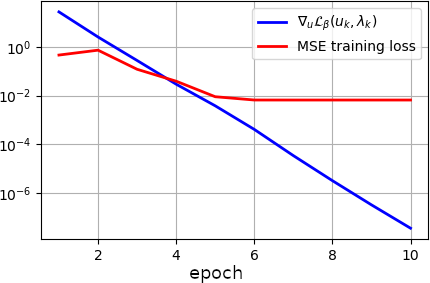
\includegraphics[width=.7\textwidth]{nabla}
	\caption{Typical convergence behaviour of Algorithm \ref{algo}}
	\label{nabla}
\end{figure}

\section{Least Squares Solver}
To solve the LS problem \ref{loss} in Algorithm \ref{algo}, a Trust Region Reflective(\texttt{trf}) method is used, which is implemented in \texttt{scipy.optimize.least\_squares}. The following description is given by \texttt{scipy}: "The algorithm iteratively solves trust-region subproblems augmented by a special diagonal quadratic term and with trust-region shape determined by the distance from the bounds and the direction of the gradient."\cite{scipyls}. The \texttt{trf} method is described as being robust for both bounded and unbounded problems, and well suited for sparse Jacobians. 

The LS problem \ref{loss} is an unbounded problem for which the library recommends using a Levenberg-Marquardt method. However this method cannot handle cases where the Jacobian has more columns than rows, which can sometimes occur depending on the size of the network and the number of data points used for training. Therefore we cannot use the Levenberg-Marquardt algorithm.

To efficiently solve the least squares problem, the solver requires an analytical solution for the Jacobian, which will be explained in the next section.

\section{Jacobian}

To solve the least squares problem, the Jacobian matrix of $M_{\beta}(u,\lambda) = \begin{bmatrix} F(u)/\sqrt{\beta} \\ h(u) + \lambda/\beta \end{bmatrix}$ must be calculated. A Jacobian is the matrix of all partial derivatives of a vector valued function. In this case:

\begin{equation}
J_{M_{\beta}} = 
\begin{bmatrix}
\frac{\partial{M_{\beta}}}{\partial u_1} & 
\frac{\partial{M_{\beta}}}{\partial u_2} & ... & 
\frac{\partial{M_{\beta}}}{\partial u_n} \\
\end{bmatrix}
\end{equation}

 It has a relatively sparse structure because there are no distant connections in the neural net, each layer is only connected to the next one and the previous one. In this section the partial derivative associated with each variable will be presented.
 
 First the columns of $J_{M_{\beta}}$ associated with the weight variables will be examined:
 
\begin{equation}
	\frac{\partial{M_{\beta}}}{\partial W_k} = -z_{k,j}\sigma'_k(W_kz_{k,j}), k = 0,\ldots,L, j = 1,\ldots,n
\end{equation}

$W_k$ is a matrix of size $d_{k+1}\times(d_k+1)$, and $z_{k,j}$ are vectors of size $d_k+1$, therefore this evaluates as a 3D tensor. $W_k$ must be vectorized first to allow this derivative to be used in the Jacobian. After vectorization the dimensions of this partial derivative as a block matrix are $d_{k+1}n \times d_{k+1}(d_{k}+1)$. The last partial derivative $\frac{\partial{M_{\beta}}}{\partial W_L}$ is also multiplied by a factor $\frac{1}{\beta}$.

 Next the columns of $J_{M_{\beta}}$ associated with the states $z_k$ are examined:
 
 \begin{equation}
 	\frac{\partial{M_{\beta}}}{\partial z_k} = \begin{bmatrix} 1 \\ -W_k\sigma'_k(W_kz_k) \end{bmatrix}, k = 1,\ldots,L
 \end{equation}
 $W_k$ are as before and $z_k$ are matrices of size $(d_k+1)\times n$. The row of ones associated with the biases vector in $W_k$ is not a variable so it is excluded from the jacobian. After vectorization of $z_k$ the partial derivative has dimensions $(d_k+d_{k+1})n\times d_kn$.
 
For a fully connected neural network with identity output activation an example has been written out in Table \ref{jac-tab}. Figure \ref{jac} shows a visual representation of the matrix, where the nonzero elements have been colored black. An alternative representation, which is mathematically the same is to swap the rows corresponding to the loss function $F(u)$ to the bottom. This gives a matrix with a banded structure, which is is plotted in figure \ref{jac2}. This is the representation used in the code.


Given a feedforward network with input dimension I, an output dimension O, and it D hidden layers of width W. The weight matrixes have $I\times W + O\times W + (D-1)\times W\times W$ parameters, the bias vectors have $D\times W+O$ parameters and the state vectors have $D\times W\times N$ parameters. On the other hand $M_{\beta}(u,\lambda)$ has an output dimension of $D\times W \times N + O\times N$. The dimension of the Jacobian for this network is therefore $(D \times W\times N + O\times N)\times (D\times W\times N + O + (D+I+O)\times W + (D-1)\times W^2)$. The Jacobian scales quadratically in size with the depth of the network and the number of datapoints. It scales cubically with the width of the network. The Jacobian will be taller than it is wide when $N \geq 1 + (D+I+O)\times W/O + (D-1)\times W^2/O$. 


\begin{figure}[b]
	\centering
	\begin{subfigure}{\textwidth}
	  \centering
	  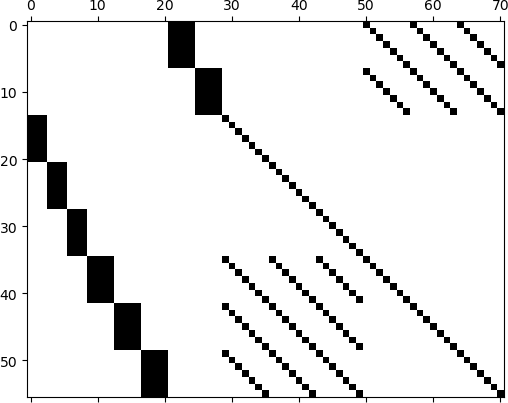
\includegraphics[width=\textwidth]{jac0.png}
	  \caption{Jacobian matrix}
	  \label{jac}
	\end{subfigure}
	\begin{subfigure}{\textwidth}
	  \centering
	  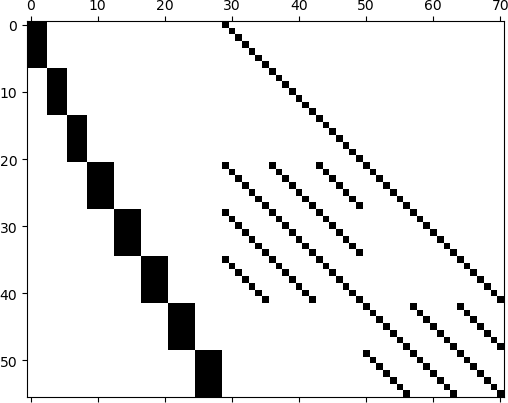
\includegraphics[width=\textwidth]{jac1.png}
	  \caption{Jacobian matrix, rearranged}
	  \label{jac2}
	\end{subfigure}
	\caption{Visual representation of Jacobian matrix for network with 2 inputs, 2 outputs, width 3, depth 2 and 7 datapoints. The non-zero elements have been colored black. The jacobian at the top is the same as the one on the bottom, but with swapped rows}
	\label{jactot}
\end{figure}

\section{Numerical verification of Jacobian Matrix}
In the previous section the Jacobian matrix was derived analytically. In this section will be explained how the Jacobian is verified algorithmically.

Algorithmic Differentation (AD) is a set of techniques which can be used to calculate the derivative of any computer code \cite{Rall1981}. Because all code is composed of elementary operations, AD can use the chain rule alongside the operations to automatically compute derivatives of arbitrary order. By injecting code from an AD library into the calculation of the neural network, the Jacobian can be calculated numerically. For this the AlgoPy python library was used. The output of the AD was then compared to the analytical result for a number of different network configurations, confirming them to be equal within a small tolerance. The code is shown in Appendix \ref{AD}

\begin{table}
\tiny
\centering

\begin{subtable}{\textwidth}
\makebox[\textwidth][c]{
\begin{tabular}{r r | c c c c c}

\multicolumn{7}{c}{Weight variables, each entry is a block matrix} \\ \hline

& $\nabla^T_{W_0,b_0}M$ & $W_{0_1}$ & $W_{0_2}$ & ... & $W_{0_W}$ & $b_0$ \\
& dim & I & I &...& I & W \\ \hline
$F$ & O*N & 0 & 0 &...& 0 & 0\\ \hline
$h_1$ & N & 		$-x\sigma'(W_{0_1}x+b_{0_1})$ & 0 &...& 0 & $-\sigma'(W_{0_1}x+b_{0_1})$ \\
      & N & 0 & 	$-x\sigma'(W_{0_2}x+b_{0_2})$ &...& 0 &  	$-\sigma'(W_{0_2}x+b_{0_2})$ \\
      &...&...&...&...&...&... \\
      & N & 0 & 0 &...& $-x\sigma'(W_{0_W}x+b_{0_W})$ &  		$-\sigma'(W_{0_W}x+b_{0_W})$ \\ \hline
$h_2$ & W*N & 0 & 0 &...& 0 & 0 \\
...   & ... &...&...&...&...&...\\ 
$h_{D}$ & W*N & 0 & 0 &...& 0 & 0 \\ \hline \\ \hline

& $\nabla^T_{W_i,b_i}M$ & $W_{i_1}$ & $W_{i_2}$ &...& $W_{i_W}$ & $b_i$ \\
& dim & W & W &...& W & W \\ \hline
$F$ & O*N & 0 & 0 &...& 0 & 0 \\ \hline
$h_1$ & W*N & 0 & 0 &...& 0 & 0 \\
...   & ... &...&...&...&...&...\\ \hline
$h_{i+1}$ & N & 		$-z_1\sigma'(W_{i_1}z + b_{i_1})$ & 0 &...& 0 & $-\sigma'(W_{i_1}x+b_{i_1})$ \\
      & N & 0 & 	$-z_1\sigma'(W_{i_2}z + b_{i_2})$ &...& 0 & 	$-\sigma'(W_{i_2}x+b_{i_2})$ \\
      &...&...&...&...&...&... \\
      & N & 0 & 0 &...& $-z_1\sigma'(W_{i_W}z + b_{i_W})$ & 		$-\sigma'(W_{i_W}x+b_{i_W})$ \\ \hline
...   & ... &...&...&...&...&...\\ 
$h_{D}$ & W*N & 0 & 0 &...& 0 & 0 \\ \hline \\ \hline

& $\nabla^T_{W_D,b_D}M$ & $W_{D_1}$ &  $W_{D_2}$  &...&  $W_{D_O}$ & $b_D$ \\
& dim & W & W &...& W & O \\ \hline
$F$ & N & $-\frac{z_D}{\sqrt{c}}\sigma_O'(W_{D_1}x+b_{D_1})$ & 0 &...& 0 & $-\frac{1}{\sqrt{c}}\sigma_O'(W_{D_1}x+b_{D_1})$ \\
    & N & 0 & $-\frac{z_D}{\sqrt{c}}\sigma_O'(W_{D_2}x+b_{D_2})$ &...& 0 & $-\frac{1}{\sqrt{c}}\sigma_O'(W_{D_2}x+b_{D_2})$ \\
      &...&...&...&...&...&... \\
    & N & 0 & 0 &...& $-\frac{z_D}{\sqrt{c}}\sigma_O'(W_{D_O}x+b_{D_O})$ & $-\frac{1}{\sqrt{c}}\sigma_O'(W_{D_O}x+b_{D_O})$ \\ \hline
$h_1$ & W*N & 0 & 0 &...& 0 & 0 \\
...   & ... &...&...&...&...&...\\ 
$h_{D}$ & W*N & 0 & 0 &...& 0 & 0 \\ \hline
      
\end{tabular}}
\end{subtable}


\begin{subtable}{\textwidth}
\makebox[\textwidth][c]{
\begin{tabular}{ r r | c c c c }
\multicolumn{6}{c}{State variables, each entry is a diagonal matrix} \\ \hline
& $\nabla^T_{z_i}M$ & $z_{i_1}$ & $z_{i_2}$ &...& $z_{i_W}$\\
&  dim & N & N &...& N \\ \hline
$F$ & O*N & 0 & 0 &...& 0 \\ \hline
$h_1$ & W*N & 0 & 0 &...& 0 \\
...   & ... &...&...&...&...\\\hline
$h_i$ & N & 1 & 0 &...& 0 \\
      & N & 0 & 1 &...& 0  \\
      &...&...&...&...&...\\ 
      & N & 0 & 0 &...& 1  \\ \hline
$h_{i+1}$ & N & $-W_{i_{1,1}}\sigma'(W_{i_1}z_i+b_{i_1})$ & $-W_{i_{1,2}}\sigma'(W_{i_1}z_i+b_{i_1})$ &...& $-W_{i_{1,W}}\sigma'(W_{i_1}z_i+b_{i_1})$\\
          & N & $-W_{i_{2,1}}\sigma'(W_{i_2}z_i+b_{i_2})$ & $-W_{i_{2,2}}\sigma'(W_{i_2}z_i+b_{i_2})$ &...& $-W_{i_{2,W}}\sigma'(W_{i_2}z_i+b_{i_2})$\\
      &...&...&...&...&...\\ 
          & N & $-W_{i_{W,1}}\sigma'(W_{i_W}z_i+b_{i_W})$ & $-W_{i_{W,2}}\sigma'(W_{i_W}z_i+b_{i_W})$ &...& $-W_{i_{W,W}}\sigma'(W_{i_W}z_i+b_{i_W})$\\ \hline
...   & ... &...&...&...&...\\ 
$h_{D}$ & W*N & 0 & 0 &...& 0 \\ \hline \\
& $\nabla^T_{z_D}M$ & $z_{D_1}$ & $z_{D_2}$ &...& $z_{D_W}$\\
& dim & N & N & ... &  N \\ \hline
F & N &         $-W_{D_{1,1}}\sigma_O'(W_{D_1}z_D+b_{D_1})$ & $-W_{D_{1,2}}\sigma_O'(W_{D_1}z_D+b_{D_1})$ &...& $-W_{D_{1,W}}\sigma_O'(W_{D_1}z_D+b_{D_1})$\\
          & N & $-W_{D_{2,1}}\sigma_O'(W_{D_2}z_D+b_{D_2})$ & $-W_{D_{2,2}}\sigma_O'(W_{D_2}z_D+b_{D_2})$ &...& $-W_{D_{2,W}}\sigma_O'(W_{D_2}z_D+b_{D_2})$\\
      &...&...&...&...&...\\ 
          & N & $-W_{D_{O,1}}\sigma_O'(W_{D_O}z_D+b_{D_O})$ & $-W_{D_{O,2}}\sigma_O'(W_{D_O}z_D+b_{D_O})$ &...& $-W_{D_{O,W}}\sigma_O'(W_{D_O}z_D+b_{D_O})$\\ \hline
$h_1$ & W*N & 0 & 0 &...& 0 \\
...   & ... &...&...&...&...\\\hline
$h_D$ & N & 1 & 0 &...& 0 \\
      & N & 0 & 1 &...& 0  \\
      &...&...&...&...&...\\ 
      & N & 0 & 0 &...& 1  \\ \hline
\end{tabular}}
\end{subtable}
\caption{Jacobian of feedforward neural network. In this table the biases are not included in the weight matrices $W_k$. Each layer has a the same width $W$ and same activation $\sigma$. There are $D$ layers. The input dimension is $I$ and the output dimension is $O$. There are $N$ datapoints.}
\label{jac-tab}

\end{table}
\FloatBarrier
\section{Conclusion}
In this chapter an Augmented Lagrangian framework was proposed to solve the Optimal Control Problem. A Least Squares solver was applied to the LS problem at the heart of the algorithm, and a Jacobian Matrix was analytically derived which is supplied to the solver. The Jacobian was also algorithmically verified. In the next chapter the algorithm will be investigated using numerical tests and compared against an industry standard optimizer.




% ... en zo verder tot
\chapter{The Final Chapter}
\label{cha:n}
\lipsum[79]

\section{The First Topic of this Chapter}
\subsection{Item 1}
\subsubsection{Sub-item 1}
\lipsum[80]

\subsubsection{Sub-item 2}
\lipsum[81]

\subsection{Item 2}
\lipsum[82]

\section{The Second Topic}
\lipsum[83-85]

\section{Conclusion}
\lipsum[86-88]

%%% Local Variables: 
%%% mode: latex
%%% TeX-master: "thesis"
%%% End: 

\chapter{Conclusion}
\label{cha:conclusion}
The main goal of this thesis was to present a novel algorithm for training deep neural networks, using methods commonly used in Optimal Control Theory. The optimization problem of neural network training was reformulated into an Optimal Control Problem. In a first step the direct multiple shooting method was applied to the OCP, which is commonly used in control theory for very nonlinear problems. 

This method was implemented in MATLAB using a very general optimization function \texttt{fmincon}, proving that the problem was feasible. Then an Augmented Lagrangian Method was presented to solve the OCP. First a textbook ALM method was implemented, later this was improved by using an inexact ALM detailed in \cite{}. The Jacobian matrix at the center of the ALM was verified to be correct using automatic differentiation tools. This ALM method was then written into code using python with \texttt{numpy},\texttt{scipy}, and \texttt{keras}

Finally the novel algorithm was tested against industry standard backpropagation methods, ADAM and SGD. It compares favorably for some smaller, harder training problems. (SPECIFY) However it scales poorly for larger datasets. As the title indicates, the original goal of this new algorithm was to better avoid "bad" local minima in training. But the new algorithm does not show much improvement compared to standard methods, and practice has shown that is not a common problem. In larger neural networks, experts suspect local minima usually have comparable performance to the global minimum \cite{Goodfellow-et-al-2016}.  


TODO: Batch approach. It also cannot yet handle loss functions besides MSE, which could be the topic of further research.




%%% Local Variables: 
%%% mode: latex
%%% TeX-master: "thesis"
%%% End: 


% Indien er bijlagen zijn:
\appendixpage*          % indien gewenst
\appendix
\chapter{De eerste bijlage}
\label{app:A}
In de bijlagen vindt men de data terug die nuttig kunnen zijn voor de
lezer, maar die niet essentieel zijn om het betoog in de normale tekst te
kunnen volgen. Voorbeelden hiervan zijn bronbestanden,
configuratie-informatie, langdradige wiskundige afleidingen, enz.

In een bijlage kunnen natuurlijk ook verdere onderverdelingen voorkomen,
evenals figuren en referenties\cite{h2g2}.

\section{Meer lorem}
\lipsum[50]

\subsection{Lorem 15--17}
\lipsum[15-17]

\subsection{Lorem 18--19}
\lipsum[18-19]

\section{Lorem 51}
\lipsum[51]

%%% Local Variables: 
%%% mode: latex
%%% TeX-master: "masterproef"
%%% End: 

% ... en zo verder tot
\chapter{De laatste bijlage}
\label{app:n}
In de bijlagen vindt men de data terug die nuttig kunnen zijn voor de
lezer, maar die niet essentieel zijn om het betoog in de normale tekst te
kunnen volgen. Voorbeelden hiervan zijn bronbestanden,
configuratie-informatie, langdradige wiskundige afleidingen, enz.

\section{Lorem 20-24}
\lipsum[20-24]

\section{Lorem 25-27}
\lipsum[25-27]

%%% Local Variables: 
%%% mode: latex
%%% TeX-master: "masterproef"
%%% End: 


\backmatter
% Na de bijlagen plaatst men nog de bibliografie.
% Je kan de  standaard "abbrv" bibliografiestijl vervangen door een andere.
\bibliographystyle{abbrv}
\bibliography{references}

\end{document}

%%% Local Variables: 
%%% mode: latex
%%% TeX-master: t
%%% End: 
